%%
% This is an Overleaf template for presentations
% using the TUM Corporate Desing https://www.tum.de/cd
%
% For further details on how to use the template, take a look at our
% GitLab repository and browse through our test documents
% https://gitlab.lrz.de/latex4ei/tum-templates.
%
% The tumbeamer class is based on the beamer class.
% If you need further customization please consult the beamer class guide
% https://ctan.org/pkg/beamer.
% Additional class options are passed down to the base class.
%
% If you encounter any bugs or undesired behaviour, please raise an issue
% in our GitLab repository
% https://gitlab.lrz.de/latex4ei/tum-templates/issues
% and provide a description and minimal working example of your problem.
%%


\documentclass[
  english,            % define the document language (english, german)
  aspectratio=43,    % define the aspect ratio (169, 43)
  % handout=2on1,       % create handout with multiple slides (2on1, 4on1)
  % partpage=false,     % insert page at beginning of parts (true, false)
  % sectionpage=true,   % insert page at beginning of sections (true, false)
]{tumbeamer}


% load additional packages
\usepackage{booktabs}


% presentation metadata
\title{Time stepping review of open-source solvers}
\subtitle{Guided research}
\author{\theAuthorName}

% \institute{\theChairName\\\theDepartmentName\\\theUniversityName}


\date{
    \small

\textbf{Supervisor:} Prof. Dr. Hans-Joachim Bungartz \\
\textbf{Advisor:} M.Sc. Benjamin Rodenberg \\
}

\footline{\insertauthor~|~\insertshorttitle~}


% macro to configure the style of the presentation
\TUMbeamersetup{
  title page = TUM tower,         % style of the title page
  part page = TUM toc,            % style of part pages
  section page = TUM toc,         % style of section pages
  content page = TUM more space,  % style of normal content pages
  tower scale = 1.0,              % scaling factor of TUM tower (if used)
  headline = TUM threeliner,      % which variation of headline to use
  footline = TUM default,         % which variation of footline to use
  % configure on which pages headlines and footlines should be printed
  headline on = {title page},
  footline on = {every page, title page=false},
}

% available frame styles for title page, part page, and section page:
% TUM default, TUM tower, TUM centered,
% TUM blue default, TUM blue tower, TUM blue centered,
% TUM shaded default, TUM shaded tower, TUM shaded centered,
% TUM flags
%
% additional frame styles for part page and section page:
% TUM toc
%
% available frame styles for content pages:
% TUM default, TUM more space
%
% available headline options:
% TUM empty, TUM oneliner, TUM twoliner, TUM threeliner, TUM logothreeliner
%
% available footline options:
% TUM empty, TUM default, TUM infoline


\begin{document}

\maketitle

\section{Introduction}

\subsection{Motivation}
\begin{frame}{Motivation}
\end{frame}

\subsection{Open-Source solvers}
\begin{frame}{Open-source solvers}
\vspace*{\fill}
    \begin{figure}
        \centering
        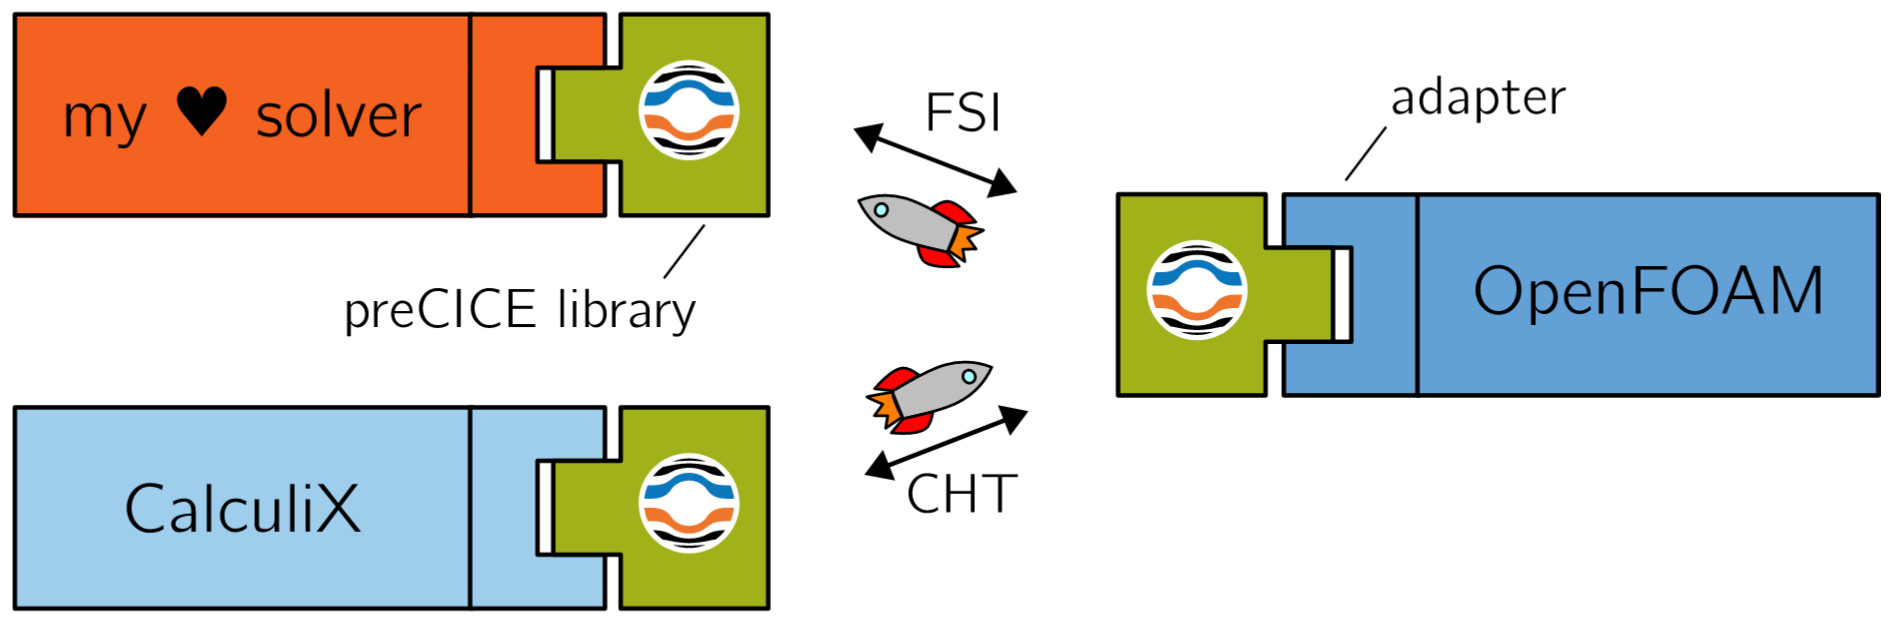
\includegraphics[width=0.9\textwidth]{resources/preCICE_graphic.png}
        \caption{Diagram showing setup for coupling simulations with preCICE library.}
        \label{fig:open-source}
    \end{figure}
% \vspace*{\fill}
\end{frame}

\subsection{Time stepping schemes}
\begin{frame}{Time stepping schemes}
When solving a PDE of the form:
\begin{equation}
    \frac{\partial u}{\partial t} = F(u, t)
\end{equation}
we need to discretize the time-derivative. Easiest way is the Euler explicit method: \\
\begin{equation}
    \frac{u^{n+1} - u^n}{\Delta t} = {F}(u^{n}, t^{n})
\end{equation}

\vspace{10pt}

We focus on second-order time stepping schemes $\rightarrow$ temporal discretization error $\varepsilon_{\Delta t}$ decreases $\mathcal{O}(\Delta t^2)$. \\
% \vspace{10pt}
% For OpenFOAM: Crank-Nicolson method \\
% \vspace{10pt}
% For CalculiX: alpha method



\end{frame}

\section{OpenFOAM}
\begin{frame}{OpenFOAM}

The error has the form $\varepsilon_u = \varepsilon_{\Delta t} + \varepsilon_{\Delta x} + \varepsilon_\text{num}$.
\vspace{10pt}

We use Crank-Nicolson time stepping method.

\vspace*{\fill}

    \begin{figure}
        \centering
        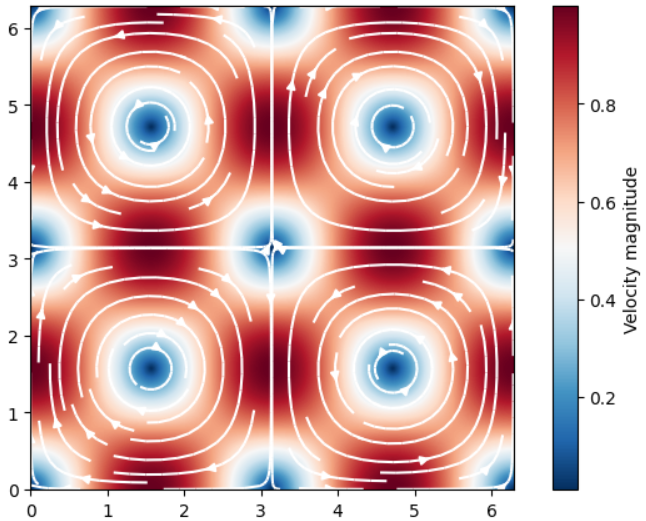
\includegraphics[width=0.5\textwidth]{resources/taylor-green-vortex.png}
        \caption{Visualization of the Taylor-Green vortex scenario.}
    \end{figure}
\end{frame}

\begin{frame}{OpenFOAM - convergence study}
\vspace*{\fill}
\begin{figure}[!htbp]
    \centering
    \begin{subfigure}[b]{0.49\textwidth}
      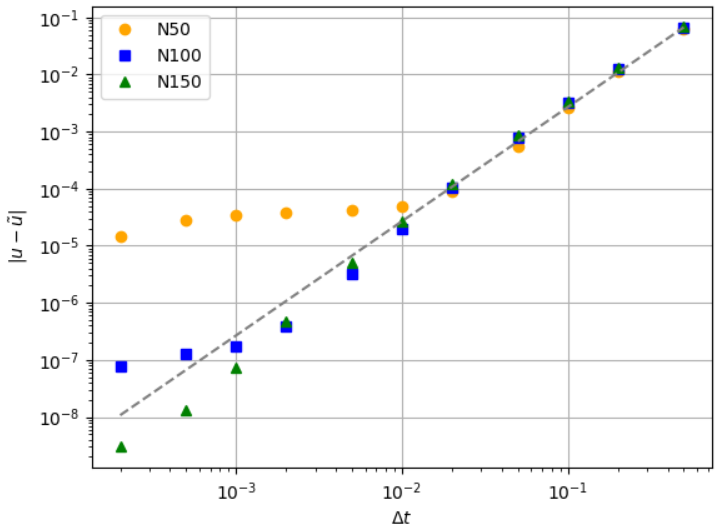
\includegraphics[width=\textwidth]{resources/ref_error_openfoam.png}
      \caption{
        Error compared to reference ($\Delta t = 10^{-5}$). \\ \\
        $|u - \tilde{u}| = \varepsilon_{\Delta t} + \varepsilon_\text{num}$ \\ \\
        plateau when $\varepsilon_{\Delta t} < \varepsilon_\text{num}$
      }
      \label{fig:convergence_openfoam}
    \end{subfigure}
    \hspace{1pt}
    \begin{subfigure}[b]{0.49\textwidth}
        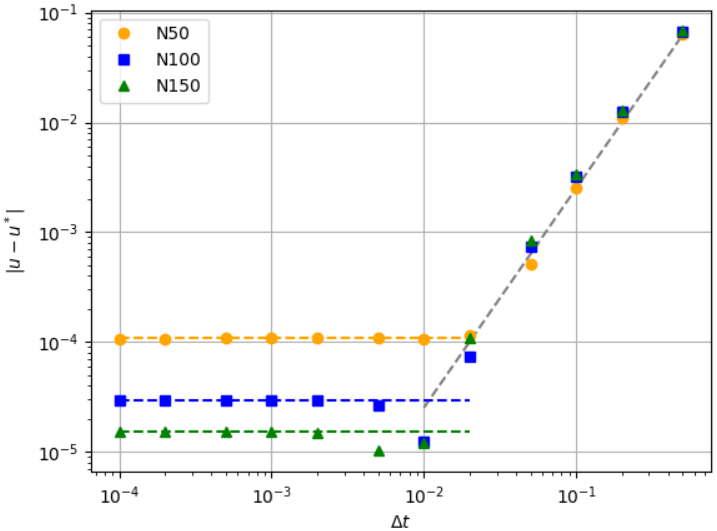
\includegraphics[width=\textwidth]{resources/analytic_error_openfoam.png}
      \caption{Error compared to analytical solution. \\ \\
      $|u - u^*| = \varepsilon_{\Delta t} + \varepsilon_{\Delta x} + \varepsilon_\text{num}$ \\ \\
      plateau when $\varepsilon_{\Delta t} < \varepsilon_{\Delta x} + \varepsilon_\text{num}$
      }
      \label{fig:RMSE_openfoam}
    \end{subfigure}
    \label{fig:figures}
  \end{figure}



\end{frame}

\section{CalculiX}
\begin{frame}{CalculiX}
We use the $\alpha$-method as time stepping scheme.

\begin{figure}[!ht]
    \centering
    \begin{subfigure}[b]{0.5\textwidth}
        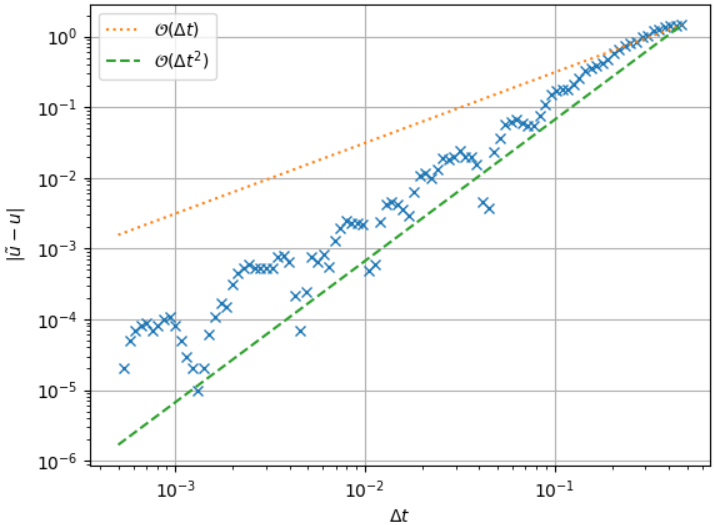
\includegraphics[width=\textwidth]{resources/calculix_convergence_study.png}
        \caption{Convergence study, showing higher-order convergence.}
    \end{subfigure}
    \hspace{0.8cm}
    \begin{subfigure}[b]{0.35\textwidth}
        \raisebox{0.11\height}{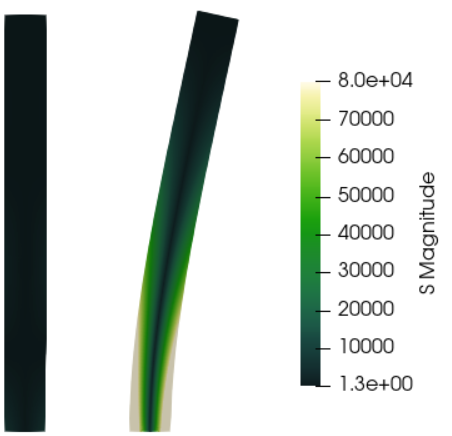
\includegraphics[width=\textwidth]{resources/elastic-flap.png}}
        \caption{Perpendicular elastic flap scenario.}
    \end{subfigure}
    \label{fig:calculix_convergence}
\end{figure}
\end{frame}

\section{FSI simulation}
\begin{frame}{FSI simulation}
\vspace*{\fill}

    \begin{figure}[!ht]
    \centering
    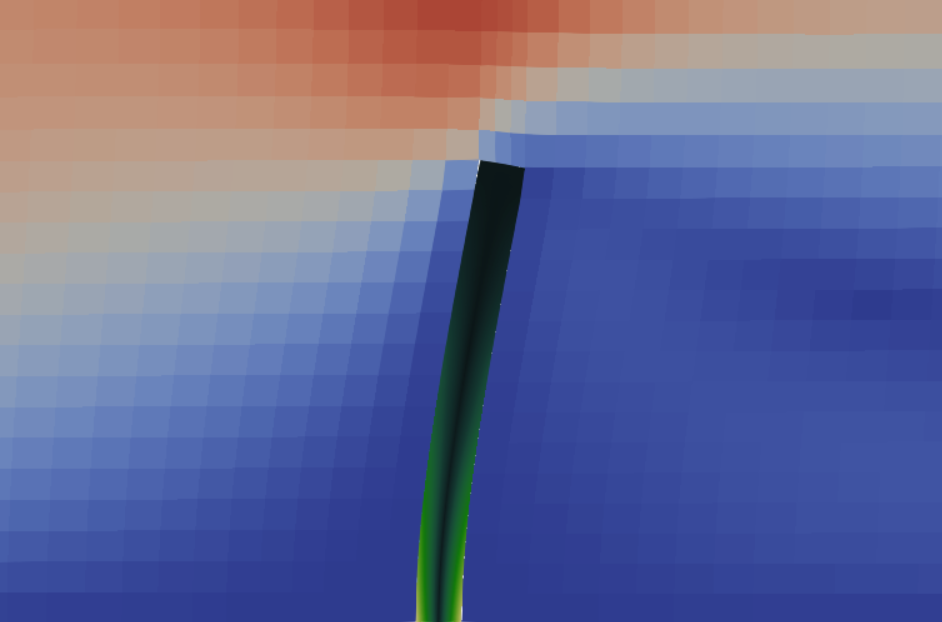
\includegraphics[width=0.45\textwidth]{resources/FSI_small.png}
    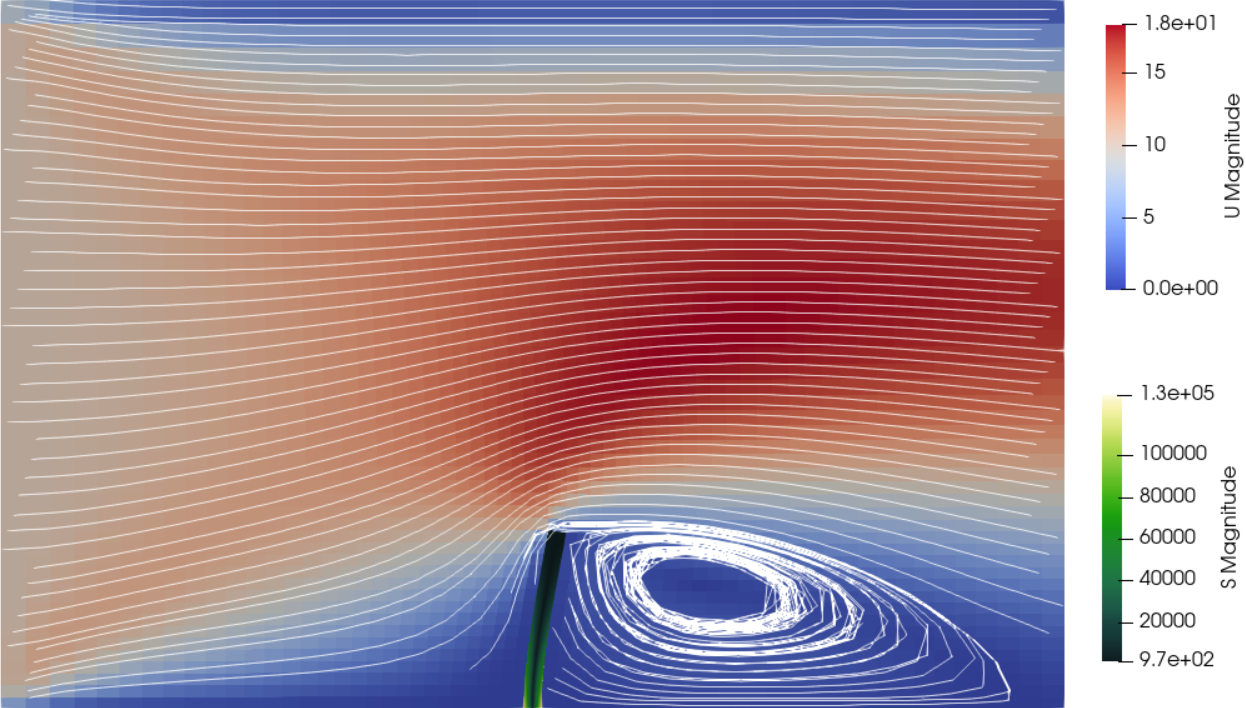
\includegraphics[width=0.523\textwidth]{resources/FSI_big.png}
    \caption{Example solution of the FSI simulation, coupled with preCICE.}
    \label{fig:FSI}
\end{figure}
\end{frame}

\begin{frame}{FSI Simulation - convergence study}
    \begin{figure}[!ht]
    \centering
    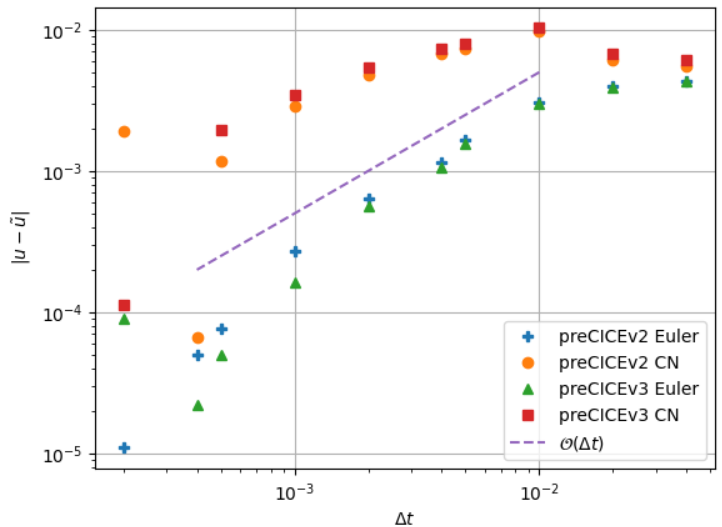
\includegraphics[width=0.6\textwidth]{resources/coupled_v2_v3_results.png}
    \caption{Convergence study of the coupled perpendicular flap scenario. Results with the Crank-Nicolson (CN) and the implicit Euler time stepping schemes, and using v2 and v3 of preCICE.}
    \label{fig:coupled_v2_v3}
\end{figure}
\end{frame}

\section{Sources of error}
\begin{frame}{Verification of CalculiX adapter}
We coupled the CalculiX adapter with a fake-fluid participant that applied a force $f^n = f_{max} \sin(t^n + \phi)$ on the tip.

\vspace*{\fill}
\begin{figure}[!ht]
    \centering
    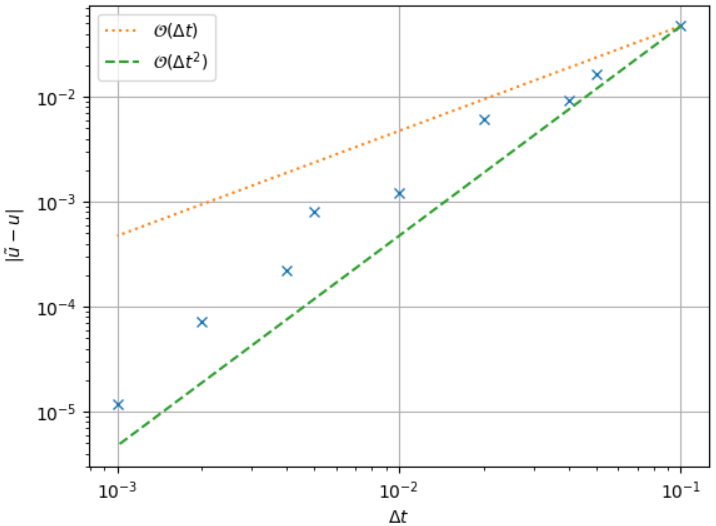
\includegraphics[width=0.57\textwidth]{resources/fake_fluid.png}
    \caption{Convergence study of the CalculiX adapter coupled with a fake fluid participant. Reference solution is $\Delta t = 10^{-4}$.}
    \label{fig:fake-fluid}
\end{figure}
\end{frame}

\begin{frame}{Verification of fluid participant}
    We ran the fluid-participant as a single-solver scenario and found: 
    \begin{itemize}
        \item Difficult convergence due to high CFL numbers.
        \item 
    \end{itemize}
\end{frame}

\section{Conclusions}
\begin{frame}{Conclusions and future work}
    \begin{itemize}
        \item Does it make sense to use second order methods? Yes, but not always.
        \vspace{15pt}
        \item Single-solver simulations showed how CalculiX and OpenFOAM can reach higher-order convergence.
        \vspace{15pt}
        \item 
        
    \end{itemize}

    
\end{frame}



\end{document}
